%********************************************************************************************
%								COMANDOS ÚTILES PARA LATEX EN ESTE TP							
%
%	\ : espacio simple
%	\\ : nueva línea
%	\par : va a la línea de abajo y deja sangría
%	\vspace{##tamaño en pt##} o \vspace{\baselineskip} en general:
%								 para dejar un espacio vertical
%	\textbf{text} :text en negrita
%	\textit{text} :text en itálica
%
% GRAFICOS CENTRADOS:
%	\begin{center}
%		\includegraphics[width=\textwidth]{./img/##ruta imagen (no hace falta extension)##}
%	\end{center}
%		--> se pueden agregar atributos como scale por si se hace muy grande
%
% TABLAS CENTRADAS:
%	\begin{center}
%	\begin{tabular}{|c|c|}
%	\hline
%	\ \textbf{Programa} & \textbf{Ticks} \\
%	\hline
%		ASM & 675127609 \\
%	\hline
%	\end{tabular}
%	\end{center}
%
% ALGORITMOS (EN VARIOS LENGUAJES):
% \begin{lstlisting}
%	void sumoDiez(int &num)
%	{
%	    num += 10;
%	}
%	
%	int main()
%	{
% 	   int i;
%	    int numeroAProcesar = 20;
%	    for (i = 0; i < 50; i++)
%	    {
%	        sumoDiez(numeroAProcesar);	//Proceso el numero en cada ciclo
%	    } 
%	    return 0;
%	}
%	\end{lstlisting}
%
% para info sobre todo lo que tiene el package detallado:
% http://en.wikibooks.org/wiki/LaTeX/Source\_Code\_Listings
%
%********************************************************************************************

\documentclass[10pt,a4paper]{article}
\usepackage[utf8]{inputenc} % para poder usar tildes en archivos UTF-8
\usepackage[spanish]{babel} % para que comandos como \today den el resultado en castellano
\usepackage{a4wide} % márgenes un poco más anchos que lo usual
\usepackage[conEntregas]{caratula}
\usepackage{amssymb}
\usepackage{fancybox}
\usepackage[usenames,dvipsnames]{color}
\usepackage{hyperref}
\usepackage{listings}
\usepackage{color}
\usepackage[table]{xcolor}
\usepackage{amsmath}
\usepackage{float}
\usepackage{pdflscape}

\hypersetup{
    colorlinks,
    citecolor=black,
    filecolor=black,
    linkcolor=black,
    urlcolor=black
}

\lstdefinestyle{customc}{
  belowcaptionskip=1\baselineskip,
  breaklines=true,
  frame=L,
  xleftmargin=\parindent,
  language=C,
  showstringspaces=false,
  basicstyle=\footnotesize\ttfamily,
  keywordstyle=\bfseries\color{green!40!black},
  commentstyle=\itshape\color{purple!40!black},
  identifierstyle=\color{blue},
  stringstyle=\color{orange},
}

\lstset{escapechar=@,style=customc}

\begin{document}

\titulo{Trabajo Práctico 1}
\subtitulo{Wiretapping}

\fecha{\today}

\materia{Teoría de las Comunicaciones}
\grupo{}

\integrante{Barbeito, Nicolás}{147/10}{nicolasbarbeiton@gmail.com}
\integrante{Garassino, Agustín Javier}{394/12}{ajgarassino@gmail.com}
\integrante{Vileriño, Silvio}{106/12}{svilerino@gmail.com}

\maketitle

\tableofcontents
\newpage

\section{Introducción}
El objetivo de este trabajo es construir una herramienta para el análisis de redes, más específicamente de la interacción de sus miembros a través de paquetes ARP (Address Resolution Protocol). Posteriormente, esta se utilizará como medio para la realización de experimentos en diversos entornos y sacar conclusiones a partir de los datos recolectados. Es decir, se recopilárá información sobre distintas redes y se tratará de deducir información significante para cada una de ellas a partir de su tráfico de paquetes ARP.

\section{Desarrollo}
\subsection{Herramienta desarrollada para análisis de la red}
\subsubsection{Motivaci\'on: Protocolo ARP}
Hoy en día la mayoría de los dispositivos con acceso a la red poseen al menos dos direcciones asociadas que permiten identificarlo unívocamente y diferenciarlo del resto. La primera de ellas, denominada MAC Address o dirección física, consiste en un identificador de 6 bytes. Esta es utilizada por diversas tecnologías de capa 2 según el modelo OSI \footnote{Modelo OSI: http://www.ecma-international.org/activities/Communications/TG11/s020269e.pdf}, por ejemplo en ethernet\footnote{Ethernet: IEEE 802.3} o las redes inalámbricas\footnote{Wi-Fi: IEEE 802.11}. La segunda es llamada dirección IP: está formada por 4 bytes y opera en la capa 3 del modelo OSI. Como estas direcciones operan a distintas capas del modelo necesitan un protocolo auxiliar que asocie las direcciones de ambos tipos a una misma máquina.

\vspace{\baselineskip}
        \begin{center}
        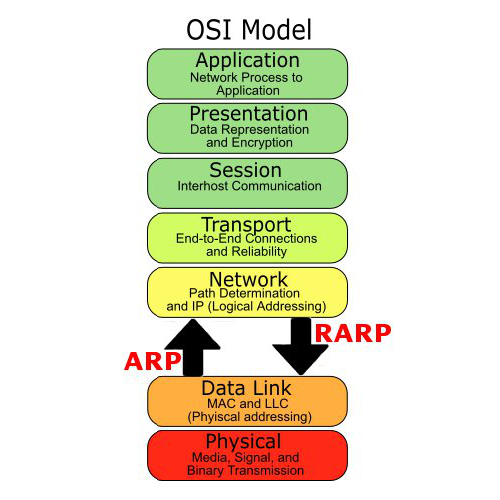
\includegraphics[scale=0.40]{fig/osimodel.jpeg}        
        \vspace{1pt}
        \footnotesize\textit{Modelo OSI. Se puede ver como el protocolo ARP se encarga de la comunicación entre la capa 2 y la capa 3.}
      \end{center}
    \vspace{\baselineskip}
\par

Es decir que el protocolo ARP surge por la necesidad de una máquina de comunicarse con otra en su misma red utilizando una tecnología de la capa nivel 2, teniendo en su poder una dirección de nivel 3. Para cumplir con su objetivo, el protocolo ARP provee dos operaciones:

\begin{itemize}
    \item \textit{who-has}: La máquina manda una señal broadcast (paquete que reciben todas las computadoras en la red) preguntando quién posee una dirección IP determinada, con el fin de obtener la MAC Address asociada.
    \item \textit{reply}: Cuando la máquina recibe un paquete ARP \textit{who-has} preguntando por su dirección, contesta únicamente al dispositivo de donde provino avisando cuál es su MAC Address.
\end{itemize}

Además cada una de las máquinas posee una tabla asociando direcciones MAC con IP de los dispositivos en la red. El propósito de esta tabla es reducir el tráfico de paquetes ARP, utilizando las operaciones solo cuando sea necesario actualizar la tabla.

\subsubsection{Implementación y uso}
La herramienta para el análisis de la red fue desarrollada en el lenguaje de programación Python, con la ayuda de diversas librerías que proveen herramientas para la manipulación de paquetes en la red \footnote{Scapy: http://www.secdev.org/projects/scapy/} y generación de visualizaciones amigables de los datos recopilados. Una vez ejecutado, el programa se encarga de filtrar los paquetes ARP que detecte en la red y obtener datos estadísticos a partir de estos. 

\section{Experimentación: Explicaci\'on}
\subsection{Enfoque del analisis}
    Se llevaron a cabo experimentos sobre varias redes distintas para analizarlas y sacar conclusiones sobre ellas. El análisis se basó considerar una red como una fuente de información y usar ciertos conceptos de la teoría clásica de información. Se usaron los dos modelos siguientes:
    $$ S_{dst} = \{s_1, \dots, s_n \} $$
    donde $s_i$ es una dirección IP que es el destino de un paquete ARP del tipo \textit{who-has}. Es decir, se considera a la dirección IP $s_i$ como un símbolo posible que la fuente $S_{dst}$ puede emitir. El otro modelo es similar:
    $$ S_{src} = \{s_1, \dots, s_n \} $$
    donde, nuevamente, $s_i$ es una dirección IP, pero en este caso es la dirección IP orígen en un paquete ARP del tipo \textit{who-has}.

\subsection{Estimaci\'on de probabilidad de aparicion de los simbolos en cada fuente}
\par Usando las herramientas desarrolladas, se capturaron paquetes ARP \textit{who-has} para estimar las probabilidades de ocurrencia de cada símbolo en las fuentes $S_{dst}$ y $S_{src}$ en cada red analizada.
Para obtener la estimaci\'on de las probabilidades de los simbolos en cada una de las fuentes, se va llevando registro de la frecuencia de aparicion $fr(s_i, f_j)$ de cada simbolo(direccion ip) $s_i$ en la fuente(red analizada)$f_j$ en una tabla \texttt{IP - Cantidad Apariciones}, luego, usando estas tablas internas(distintas para cada fuente), se obtiene la probabilidad estimada de cada simbolo $s_i$ para la fuente $f_j$ realizando el siguiente calculo $p_{(s_i, f_j)} = \frac{fr(s_i, f_j)}{N}$, siendo $N$ la cantidad de paquetes capturados en la red $f_j$.
% Para realizar esta estimación se modeló probabilidad de ocurrencia del símbolo $s_i$ (en alguna de las fuentes) con una variable binomial $Bi(k, p_{s_i})$, con $k$ la cantidad de capturas en la red y $p_{s_i}$ la probabilidad de ocurrencia del símbolo $s_i$. Luego usando las capturas, se estimó $p_{s_i}$ con el cociente $\frac{fr(s_i)}{k}$, donde $fr(s_i)$ es la cantidad de veces que se observó el símbolo $s_i$ y $k$ se definió anteriormente.
\\
\subsection{Estimaci\'on de la entropia de la fuente}
También se estimó usando la información obtenida la entropía en las redes analizadas (según los modelos anteriores), La estimaci\'on para una fuente $f_j$ fue realizada realizando el calculo $H_{(f_j)} = \sum\limits_{s_i \in simbolos(f_j)} p(s_i, f_j) * log_2(\frac{1}{p(s_i,f_j)})$.
La información que nos puede brindar este concepto es una medida de que tan centralizado está el intercambio de paquetes ARP en una red. Esto es así porque la entropía es considerada una medida de la incertidumbre del sistema, es decir, una entropía alta se interpreta como una incertidumbre alta. Esta incertidumbre en nuestro modelo es máxima cuando $p_{s_1} = \dots = p_{s_n}$, es decir cuando cualquier símbolo tiene la misma probabilidad de ser emitido por la fuente, lo que se traduce en que toda dirección IP tiene iguales probabilidades de aparecer como dirección orígen o destino (según el modelo) en un paquete ARP \textit{who-has}.
 
\subsection{Estimacion de la topologia de la red}
Con el objetivo de investigar un poco mas acerca de la red analizada, utilizando librerias gr\'aficas para python se modelo la red analizada como un grafo indicando en ella, un nodo por cada host en la red, y una arista dirigida entre $h_i$ y $h_j$ de color {\color{green}verde} si se trata de un paquete \texttt{is-at} con origen $h_i$ y destino $h_j$, asimismo, si la flecha fuera de color {\color{red}rojo} se trata de un paquete \texttt{who-has} entre los dos hosts mencionados. Dado que la interaccion entre 2 hosts puede ser m\'ultiple, se asocia un peso al eje entre ambos nodos, indicando la cantidad de paquetes de ese tipo(color) fueron enviados entre ellos. Como medida adicional para detectar nodos distinguidos, se realiza una variaci\'on del color de fondo del nodo, mientras mas cercano al (0, 0, 0) en RGB se encuentre el fondo del nodo en el gr\'afico, esto es proporcional a la cantidad de paquetes con destino a ese host existen en la red. Otra medida que nos parecio interesante explorar fue la de resolver el nombre del fabricante de la MAC Address de cada host para tener una idea adicional acerca del tipo de dispositivo, esto se ve tanto en la tabla de dispositivos resuelta como en el grafo generado.

\subsection{Aclaraciones}
Para facilitar la lectura de ambos tipos de direcciones a los humanos, generalmente las primeras son escritas como números hexadecimales separados por ':', mientras que las direcciones IP se escriben como números decimales separados por puntos. Siendo, por ejemplo, 00:22:b0:00:f2:61 una MAC Address válida y 192.168.1.10 una dirección IP.

\section{Experimentacion: Redes analizadas}
\subsection{Red domestica}
\subsubsection{Topologia estimada de red}
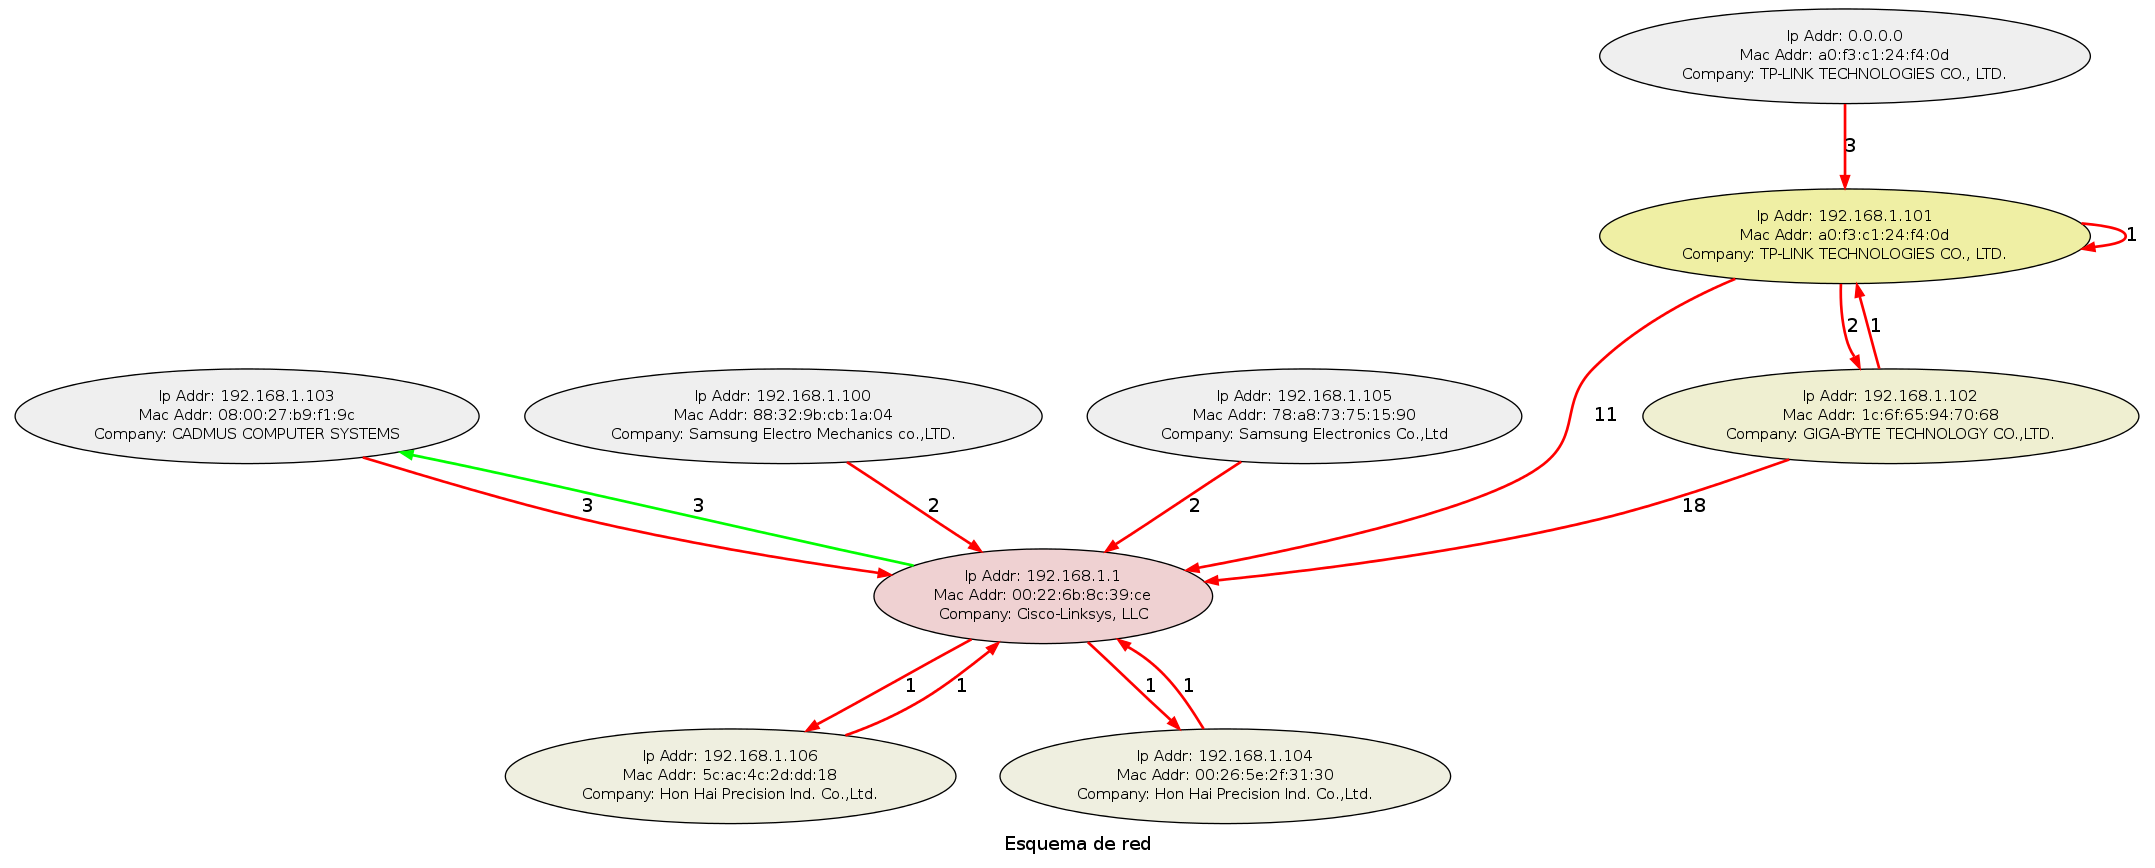
\includegraphics[scale=0.22]{../experimentacion-svilerino/casa/graph.png}

\subsubsection{Probabilidades y entropia de fuente origen}
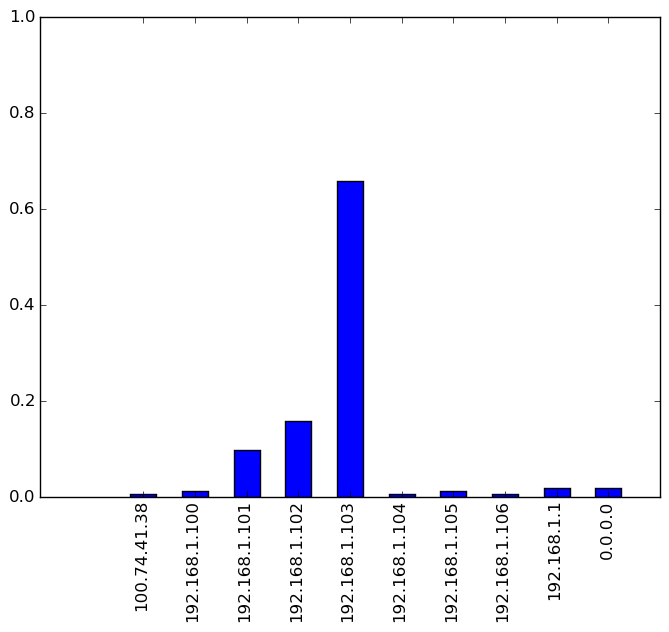
\includegraphics[scale=0.33]{../experimentacion-svilerino/casa/histogram_src_probabilities.png}
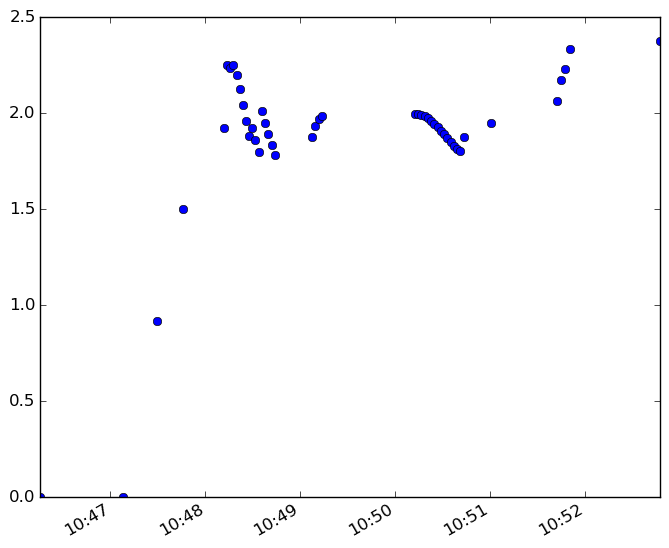
\includegraphics[scale=0.33]{../experimentacion-svilerino/casa/entropy_src.png}

\subsubsection{Probabilidades y entropia de fuente destino}
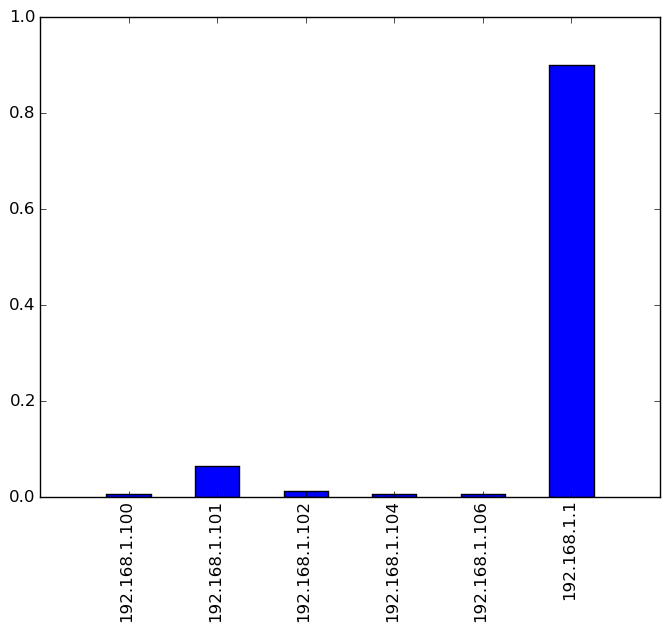
\includegraphics[scale=0.33]{../experimentacion-svilerino/casa/histogram_dst_probabilities.png}
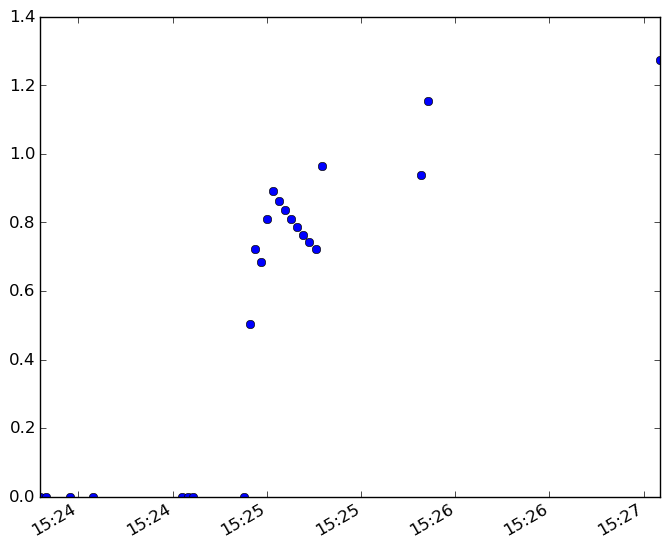
\includegraphics[scale=0.33]{../experimentacion-svilerino/casa/entropy_dst.png}

\subsubsection{Tabla de dispositivos detectados}
\lstinputlisting{../experimentacion-svilerino/casa/mac_disp_table.txt}

\subsubsection{Conclusiones del experimento} 
\subsection{Starbucks}
\subsubsection{Topologia estimada de red}
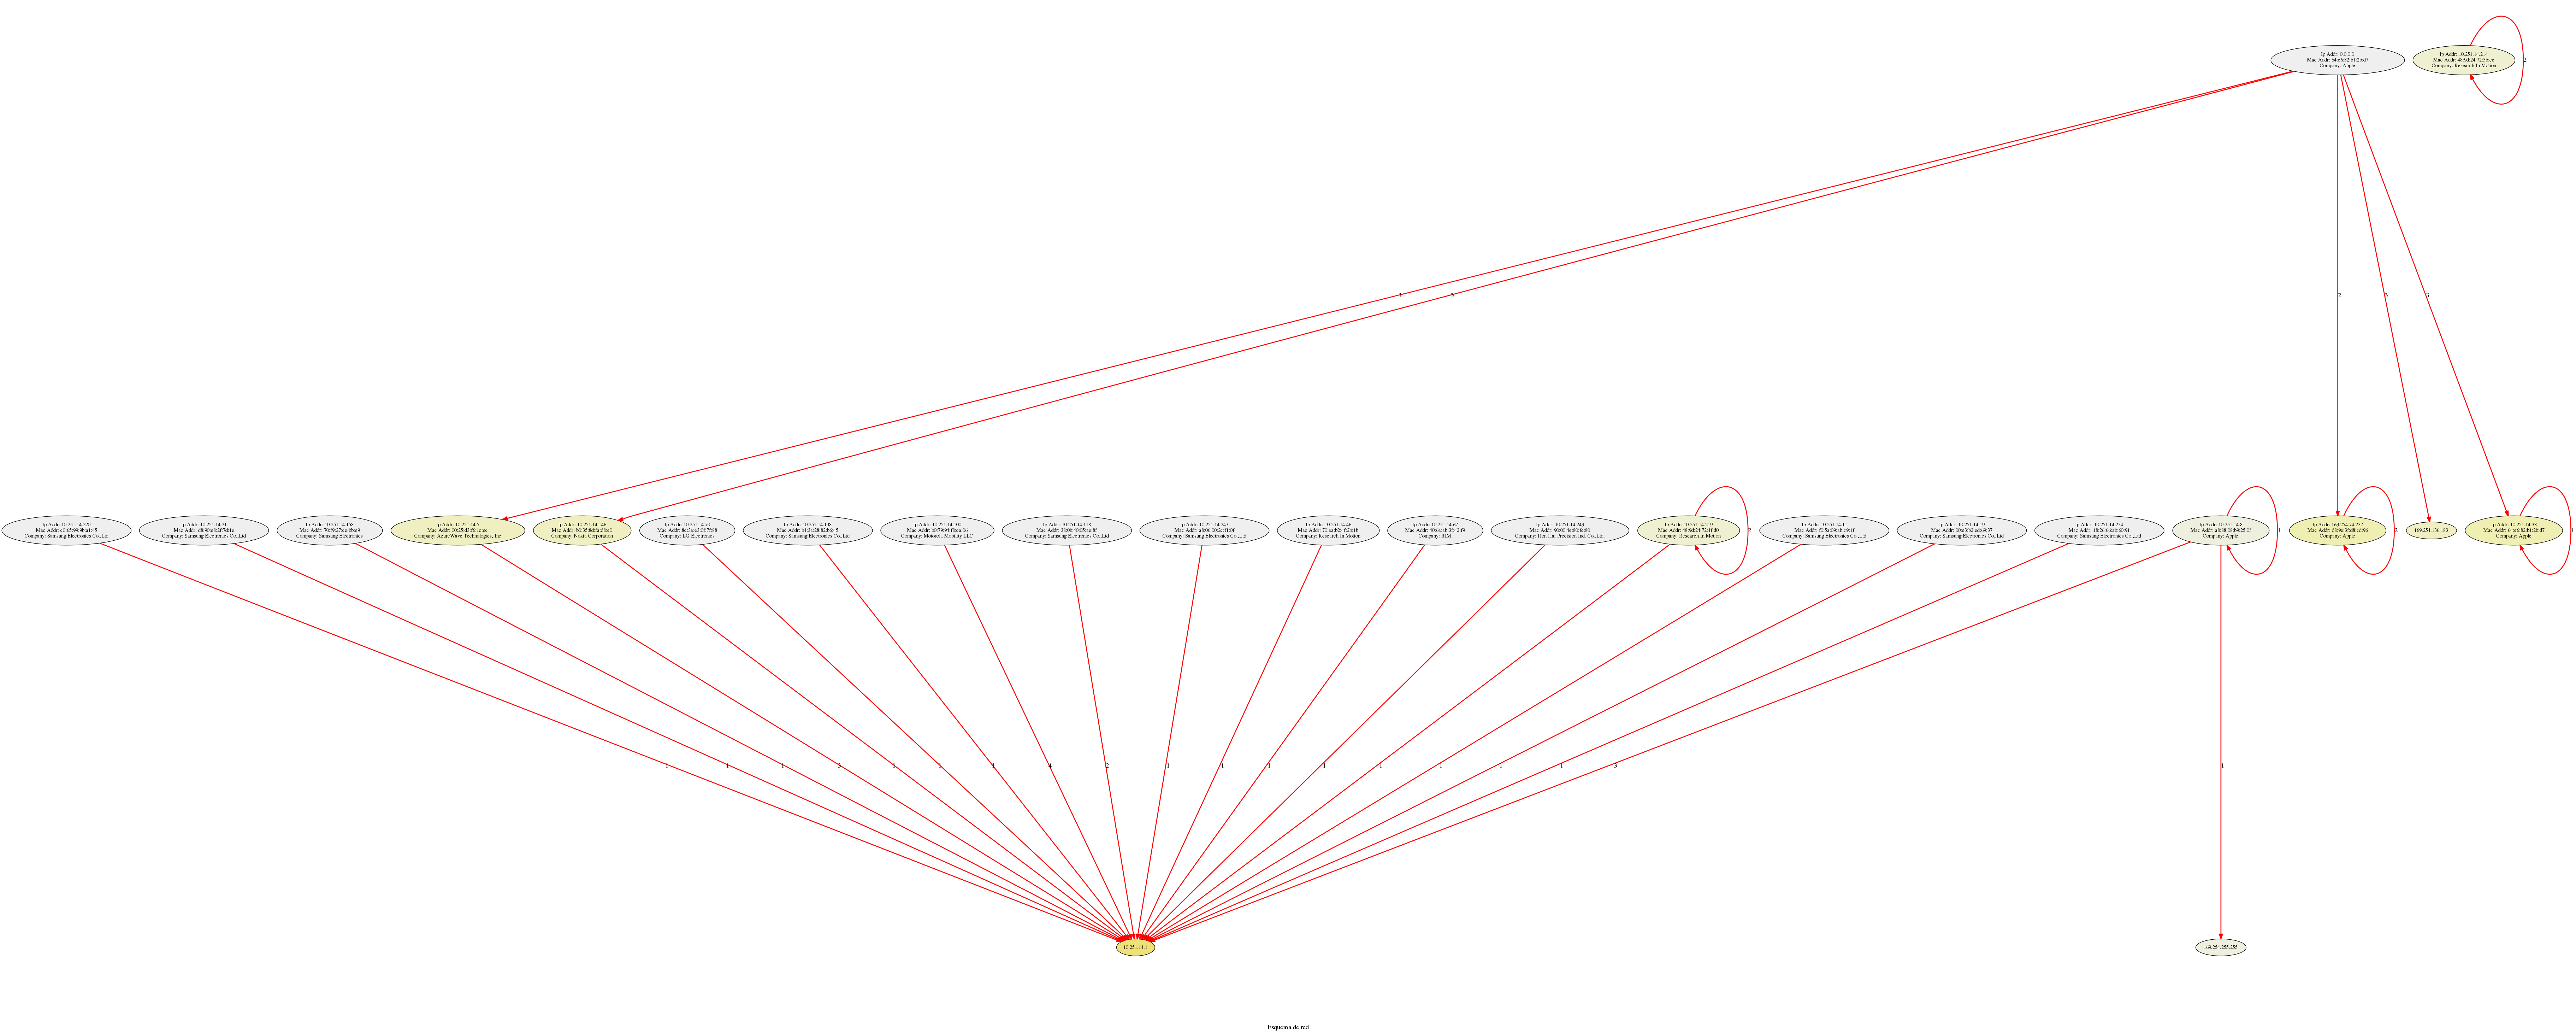
\includegraphics[scale=0.22]{../experimentacion-svilerino/starbucks/full-experiment-1/graph.png}

\subsubsection{Probabilidades y entropia de fuente origen}
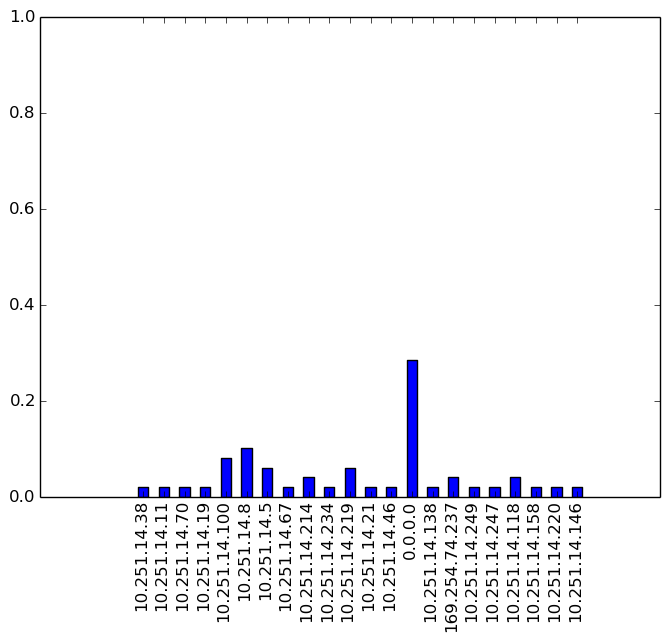
\includegraphics[scale=0.33]{../experimentacion-svilerino/starbucks/full-experiment-1/histogram_src_probabilities.png}
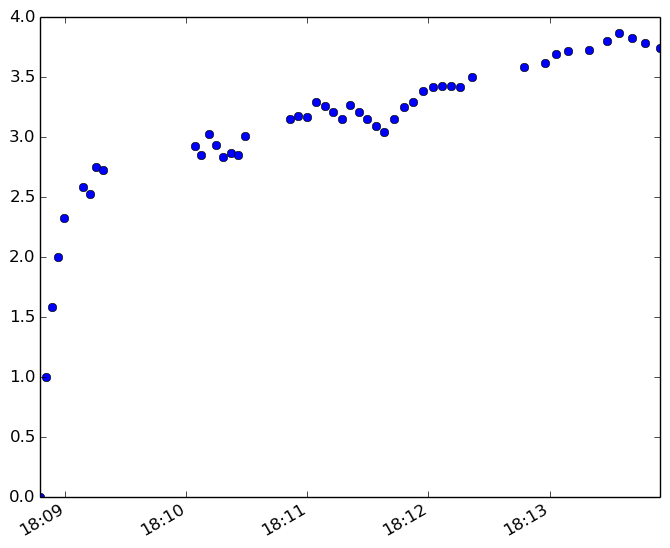
\includegraphics[scale=0.33]{../experimentacion-svilerino/starbucks/full-experiment-1/entropy_src.png}

\subsubsection{Probabilidades y entropia de fuente destino}
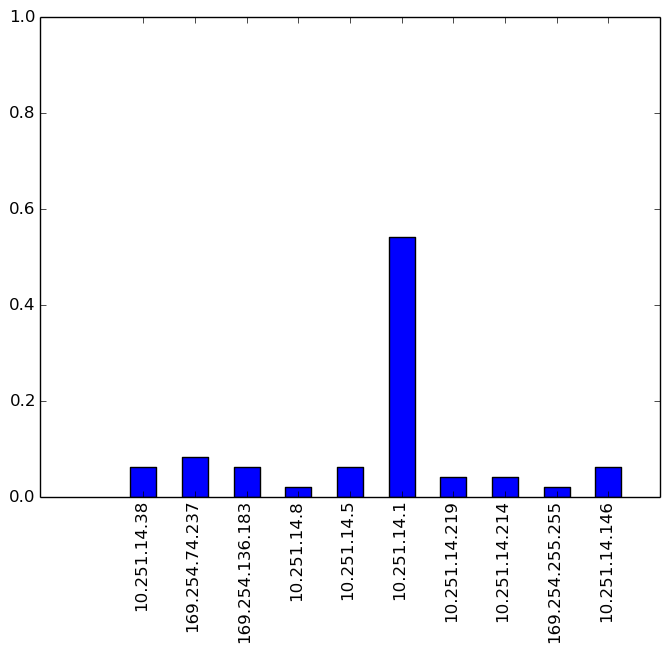
\includegraphics[scale=0.33]{../experimentacion-svilerino/starbucks/full-experiment-1/histogram_dst_probabilities.png}
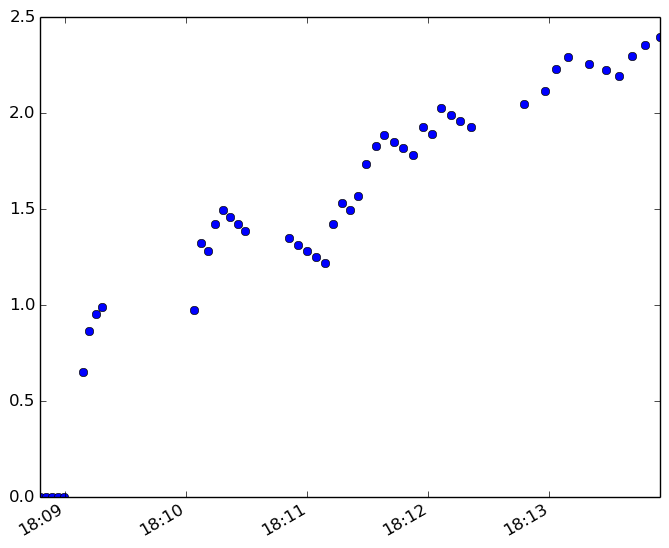
\includegraphics[scale=0.33]{../experimentacion-svilerino/starbucks/full-experiment-1/entropy_dst.png}

\subsubsection{Tabla de dispositivos detectados}
\lstinputlisting{../experimentacion-svilerino/starbucks/full-experiment-1/mac_disp_table.txt}

\huge{agregar las imagenes de los grafos alternativos mas chicos con el cisco}

\subsubsection{Conclusiones del experimento} 
%\subsection{Laboratorios del DC - WiFi1}%entrepisoDC
\subsubsection{Topologia estimada de red}
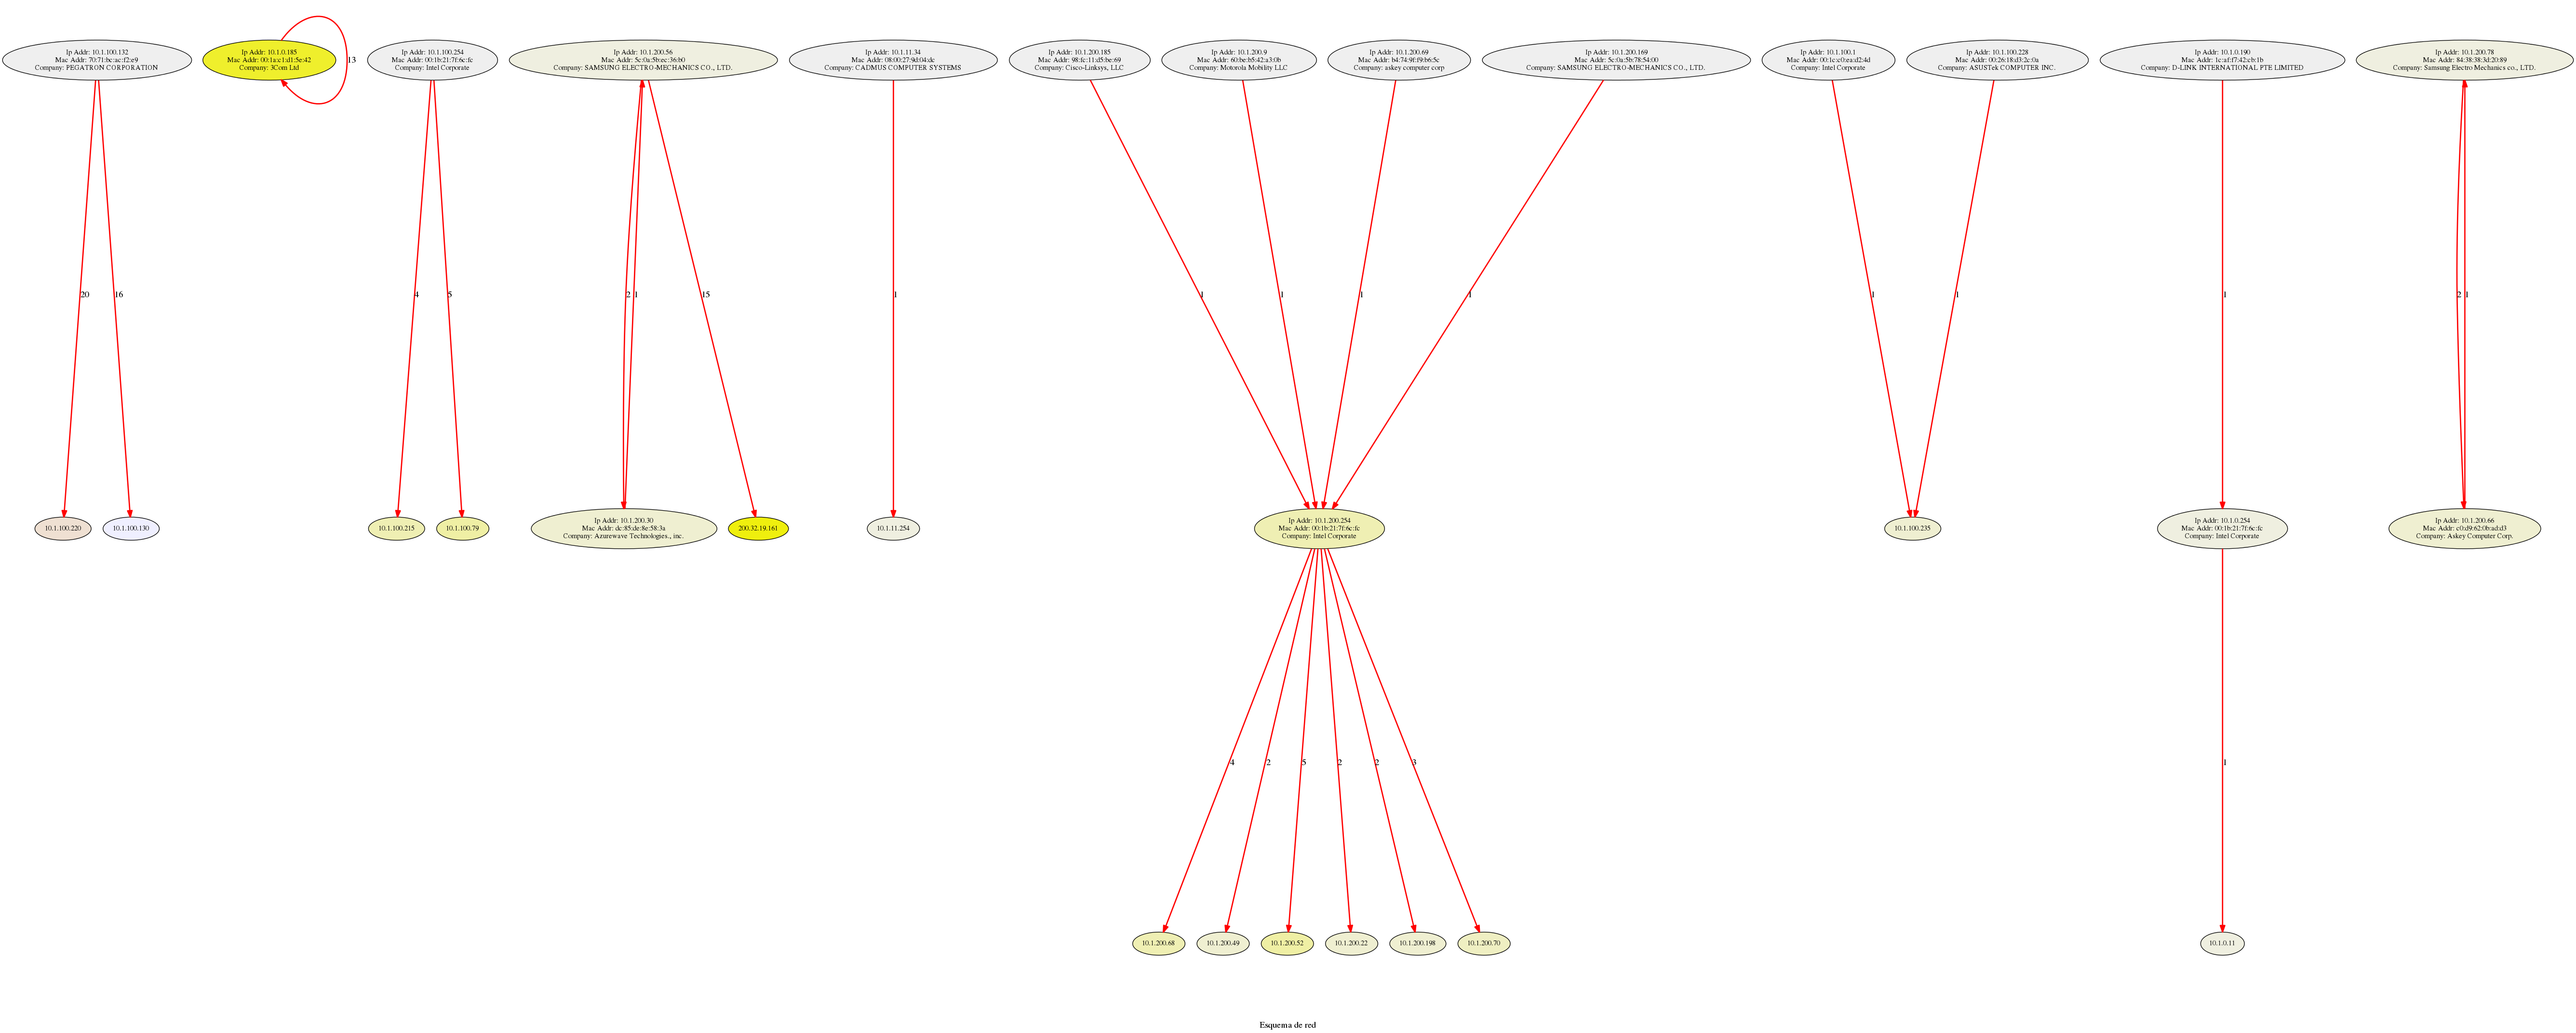
\includegraphics[scale=0.22]{../experimentacion-svilerino/labo-entrepisodc/graph.png}

\subsubsection{Probabilidades y entropia de fuente origen}
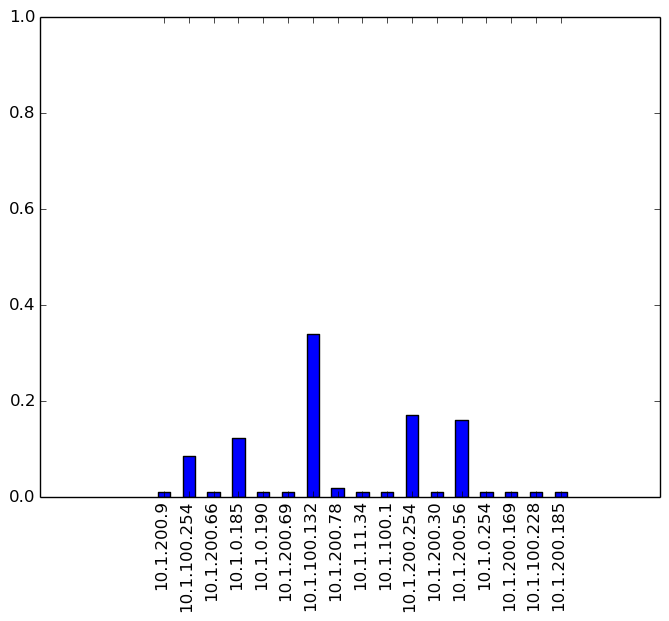
\includegraphics[scale=0.33]{../experimentacion-svilerino/labo-entrepisodc/histogram_src_probabilities.png}
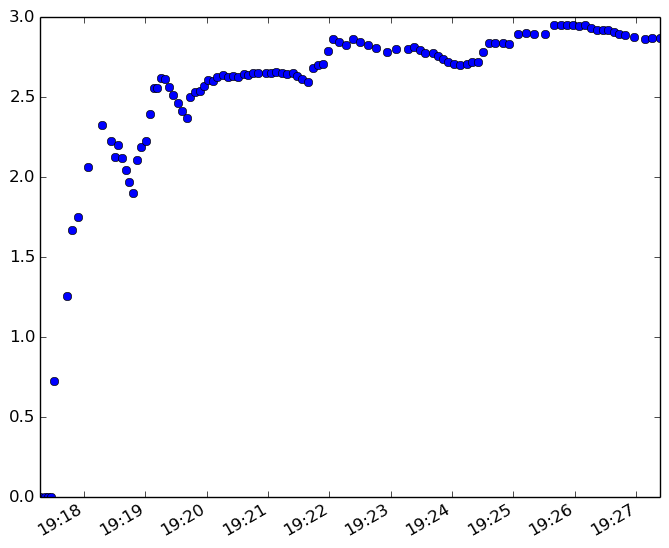
\includegraphics[scale=0.33]{../experimentacion-svilerino/labo-entrepisodc/entropy_src.png}

\subsubsection{Probabilidades y entropia de fuente destino}
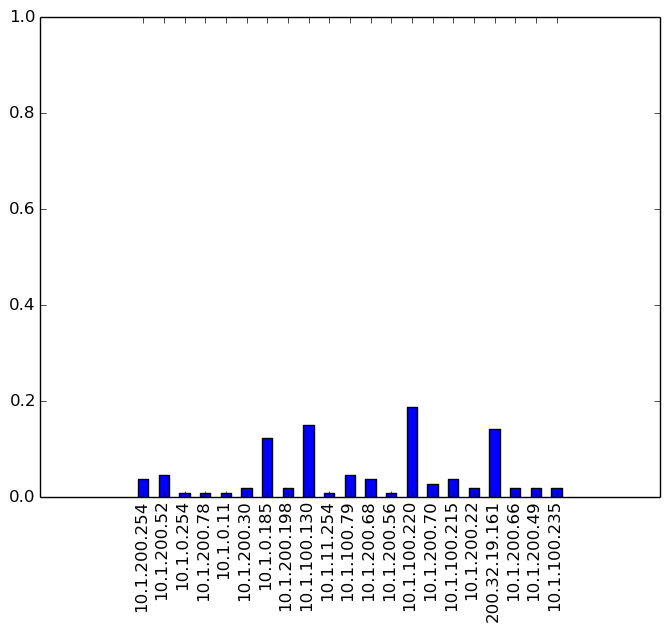
\includegraphics[scale=0.33]{../experimentacion-svilerino/labo-entrepisodc/histogram_dst_probabilities.png}
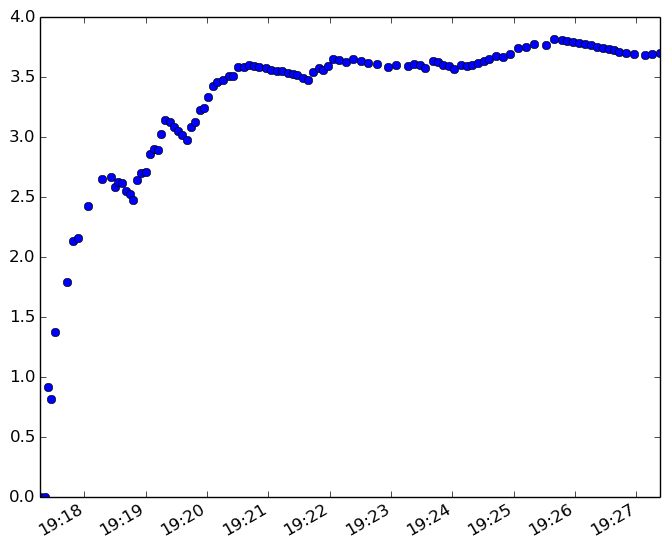
\includegraphics[scale=0.33]{../experimentacion-svilerino/labo-entrepisodc/entropy_dst.png}

\subsubsection{Tabla de dispositivos detectados}
\lstinputlisting{../experimentacion-svilerino/labo-entrepisodc/mac_disp_table.txt}

\subsubsection{Conclusiones del experimento} 
%\subsection{Laboratorios del DC - WiFi2}%licar
\subsubsection{Topologia estimada de red}
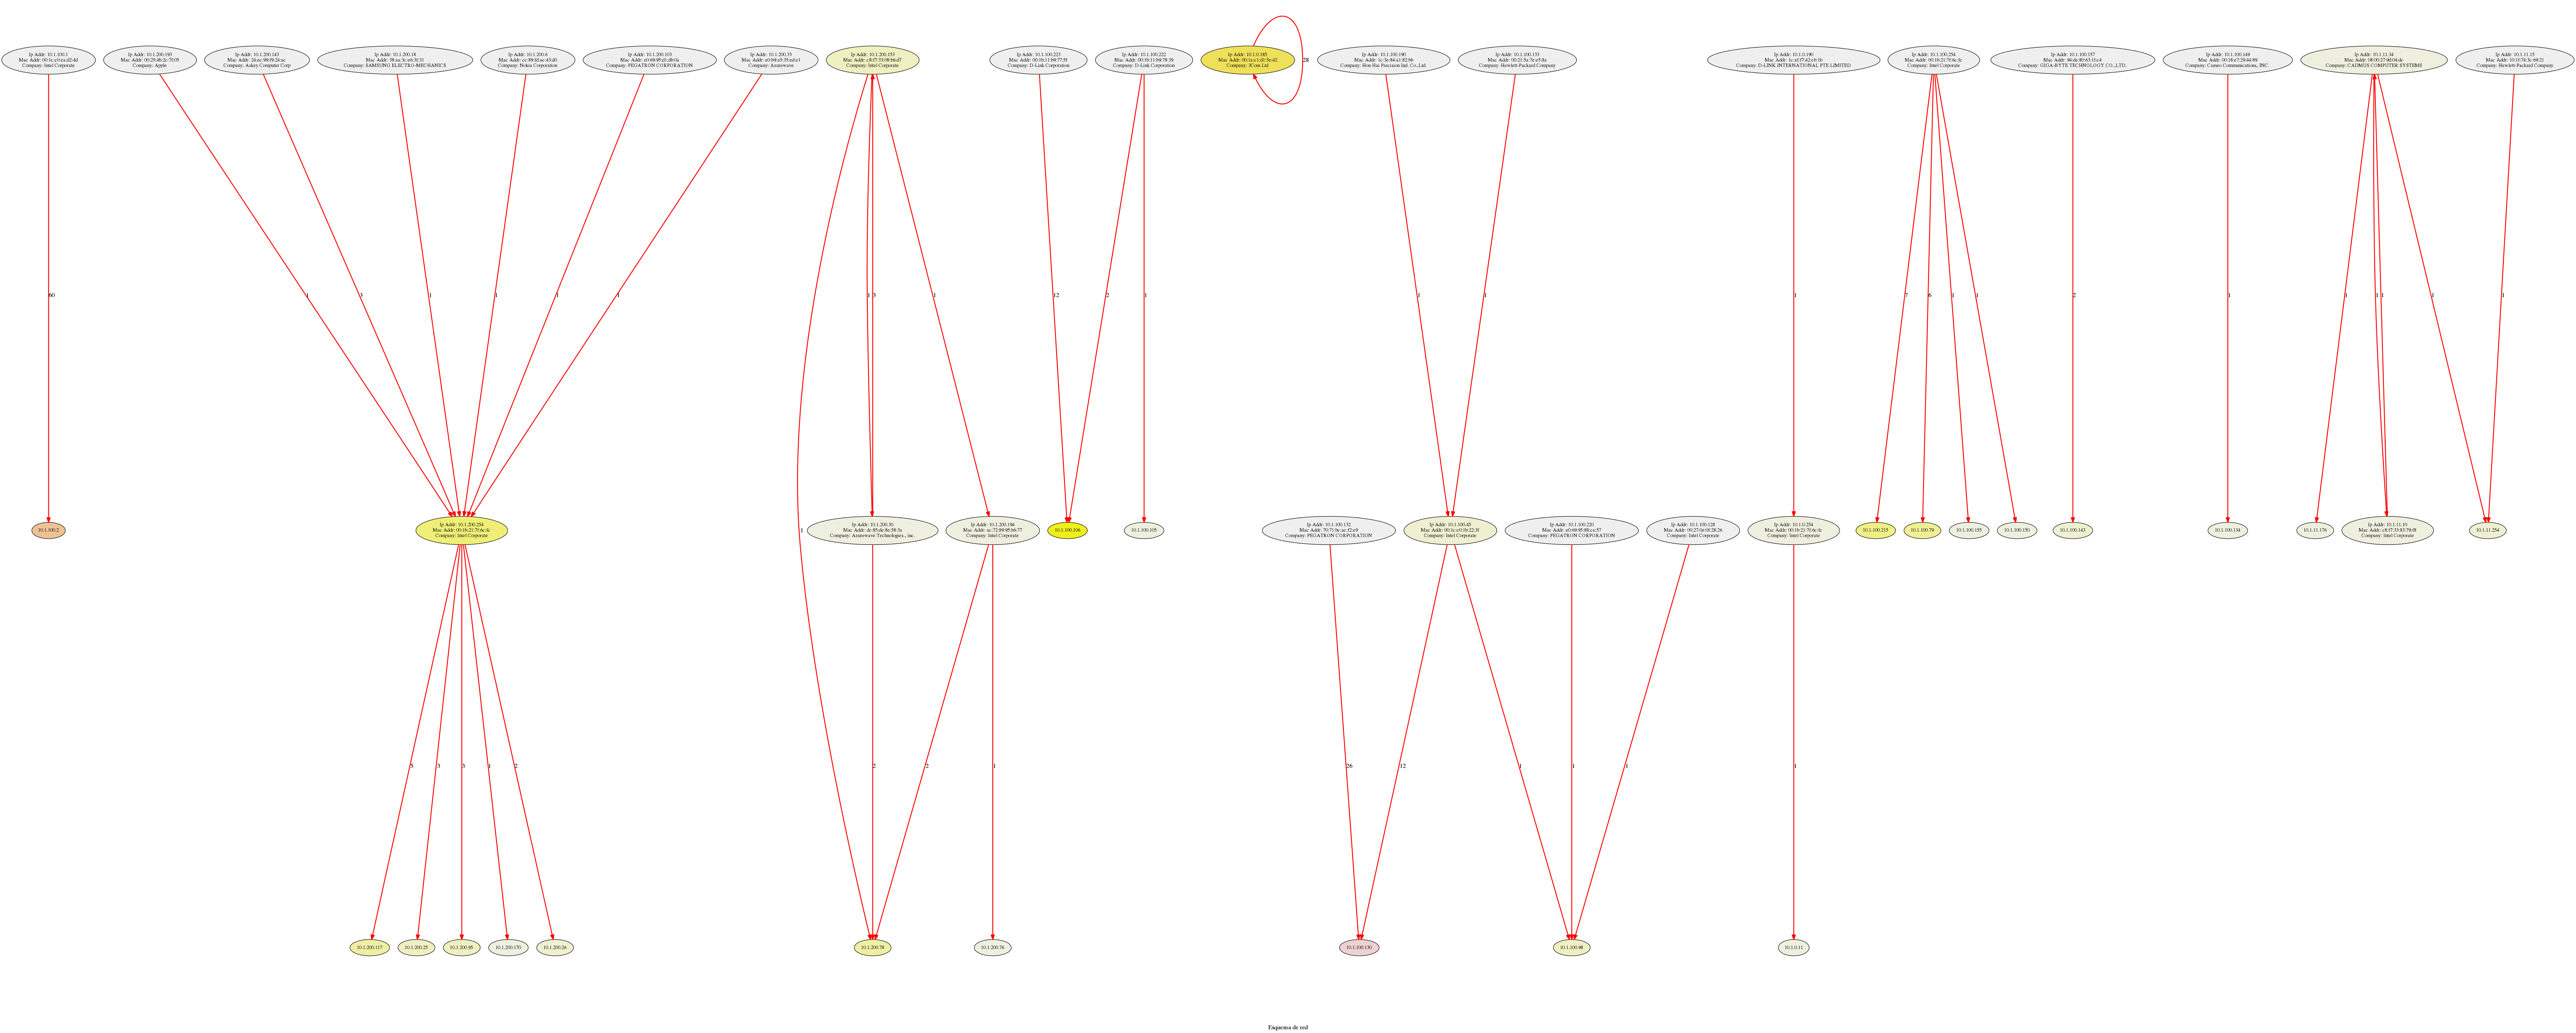
\includegraphics[scale=0.22]{../experimentacion-svilerino/licar/graph.png}

\subsubsection{Probabilidades y entropia de fuente origen}
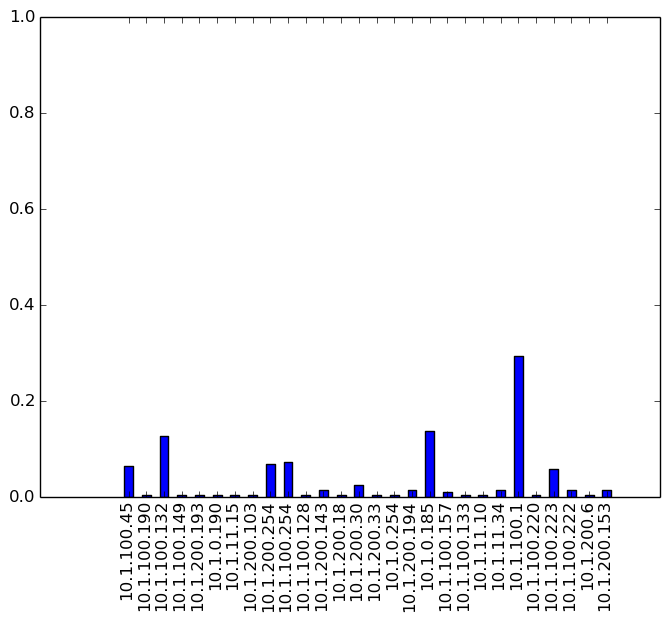
\includegraphics[scale=0.33]{../experimentacion-svilerino/licar/histogram_src_probabilities.png}
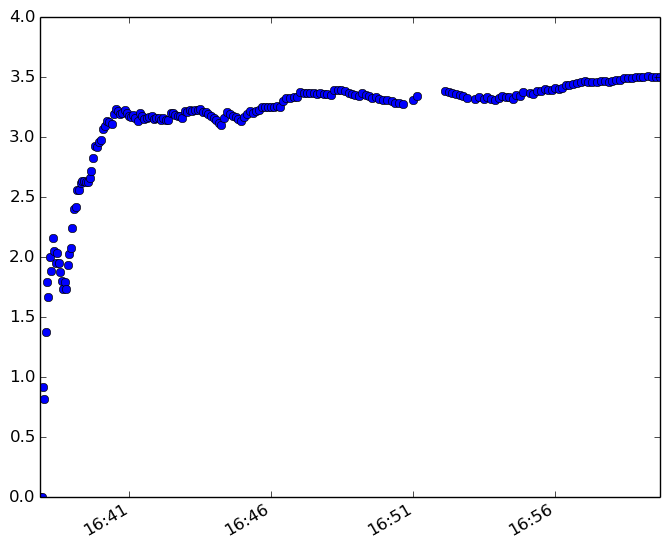
\includegraphics[scale=0.33]{../experimentacion-svilerino/licar/entropy_src.png}

\subsubsection{Probabilidades y entropia de fuente destino}
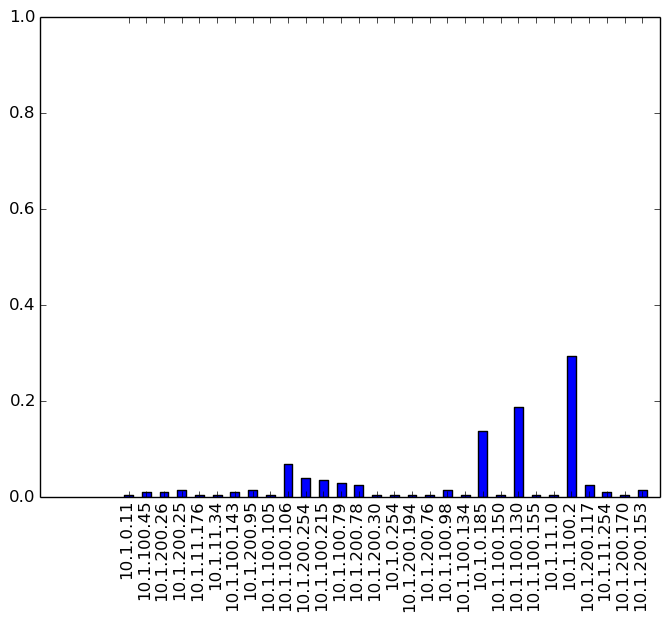
\includegraphics[scale=0.33]{../experimentacion-svilerino/licar/histogram_dst_probabilities.png}
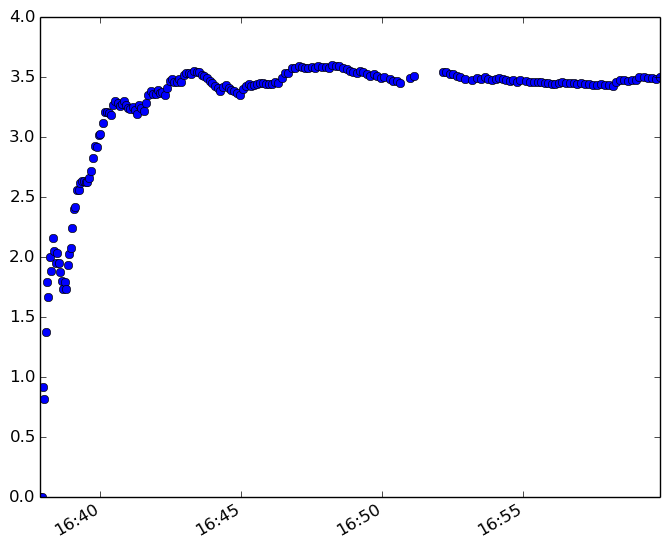
\includegraphics[scale=0.33]{../experimentacion-svilerino/licar/entropy_dst.png}

\subsubsection{Tabla de dispositivos detectados}
\lstinputlisting{../experimentacion-svilerino/licar/mac_disp_table.txt}

\subsubsection{Conclusiones del experimento} 
\subsection{Sitio de trabajo}
\subsection{Estación de servicio}
\subsubsection{Descripción del experimento}
El experimento se realizó en una estación de servicio, en la cual se ejecutó el programa de captura de paquetes ARP durante aproximadamente $46$ minutos. Los resultados y el análisis de los mismos se encuentran abajo.

\subsubsection{Resultados del experimento}

\begin{landscape}
\begin{figure}[H]
  \centering	
	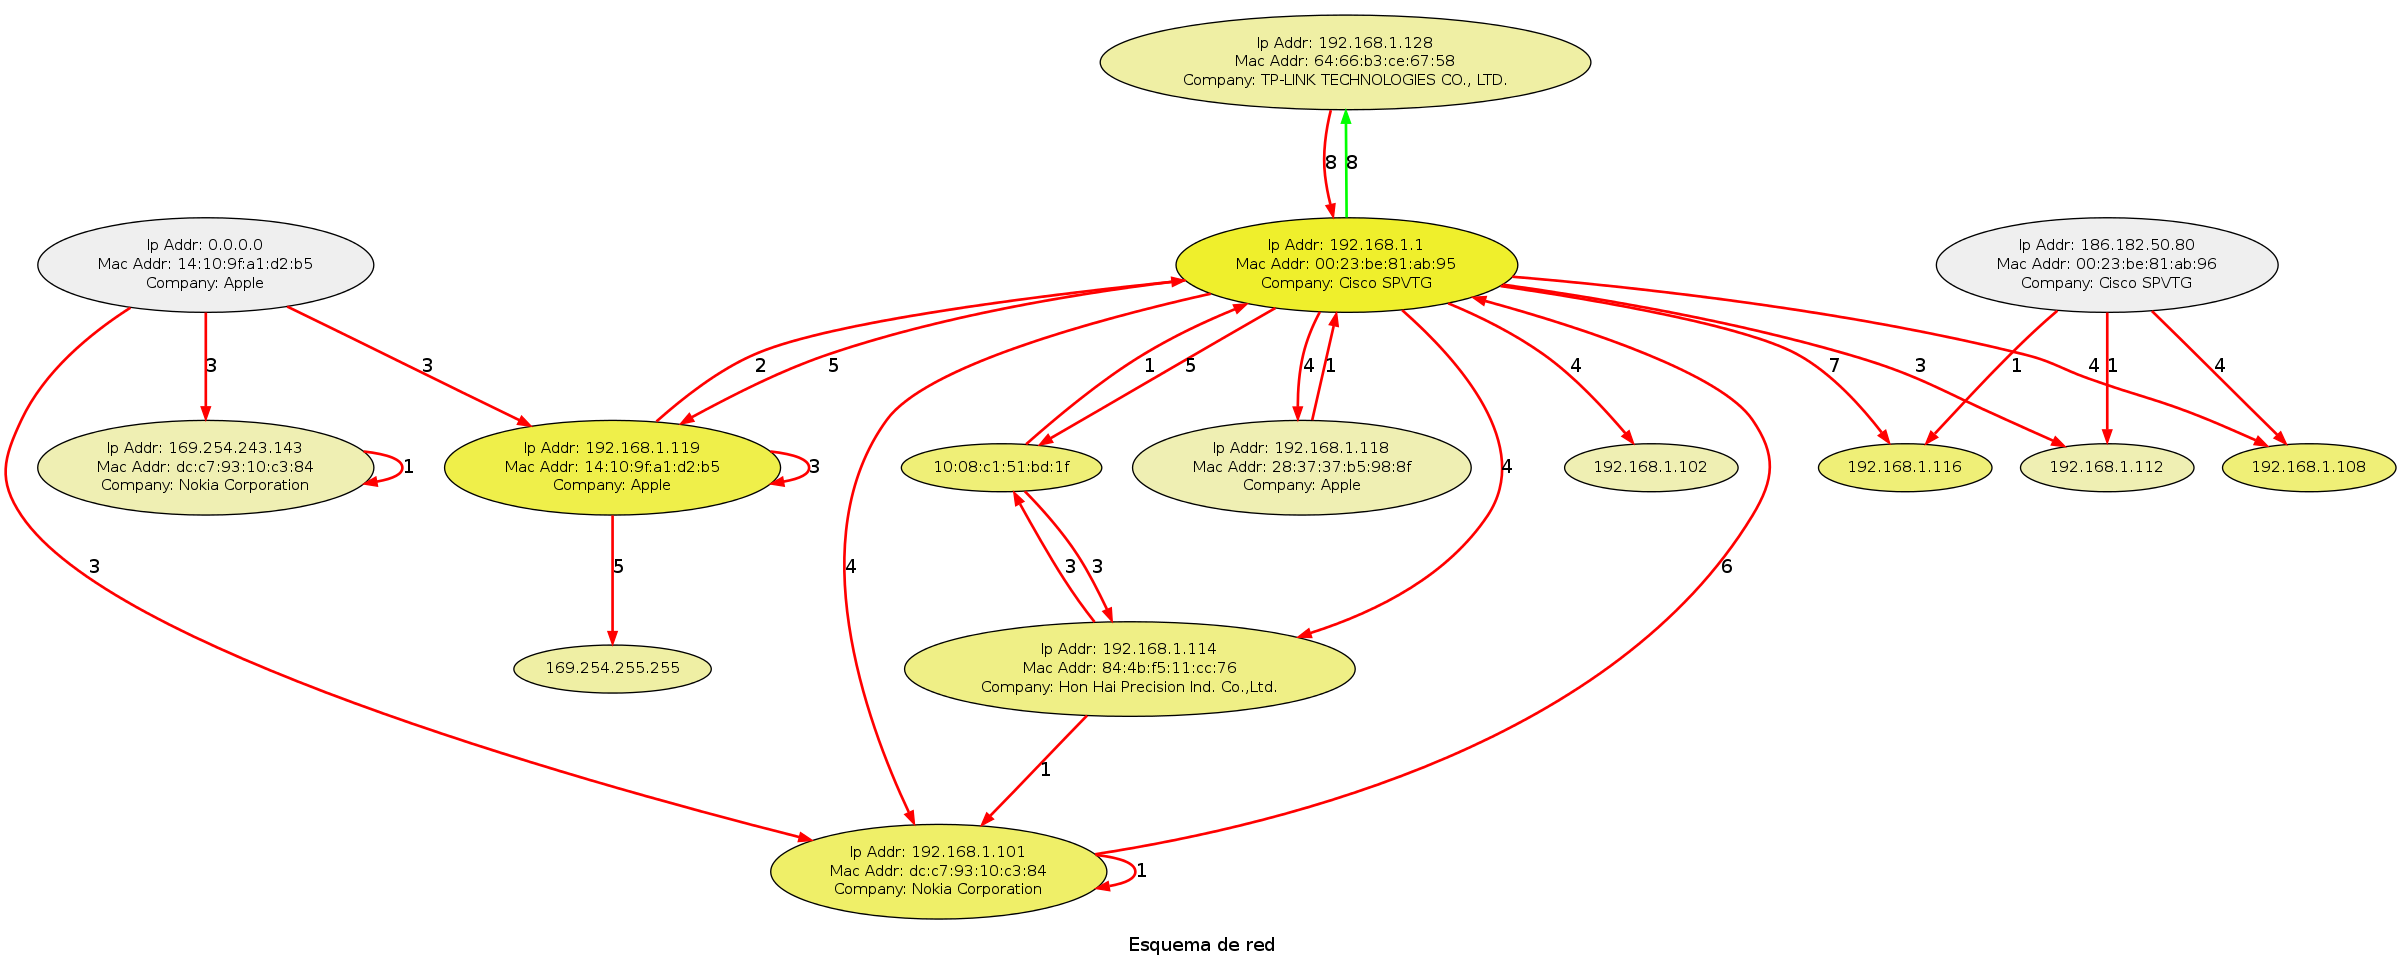
\includegraphics[scale=0.30]{../experimentacion-barbeiton/graph.png}
  \caption{Grafo de la red analizada según los paquetes ARP.}
\end{figure}
\end{landscape}

\begin{figure}[H]
  \centering	
	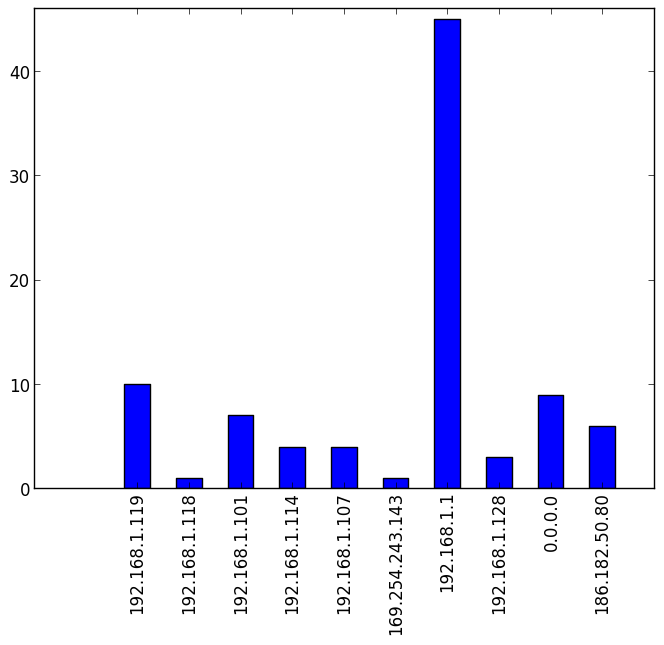
\includegraphics[scale=0.66]{../experimentacion-barbeiton/histogram_src.png}
  \caption{Histograma de las IP fuente.}
\end{figure}

\begin{figure}[H]
  \centering
	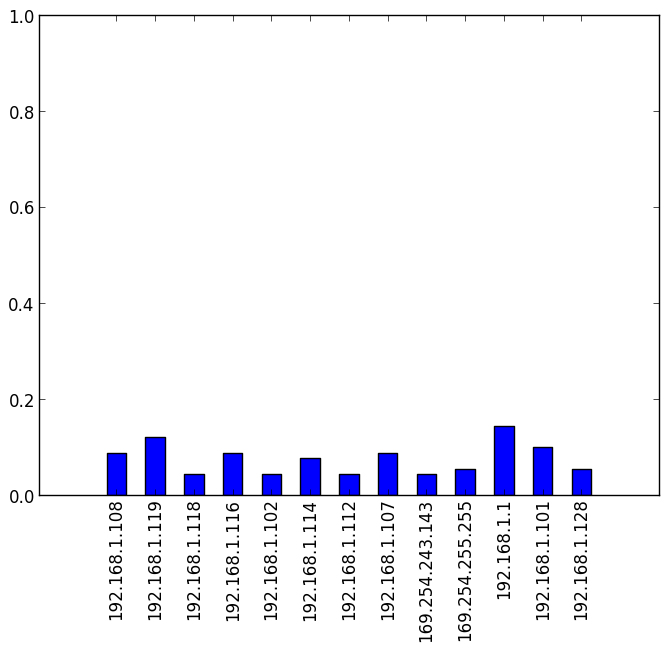
\includegraphics[scale=0.66]{../experimentacion-barbeiton/histogram_dst_probabilities.png}
  \caption{Probabilidades asociadas a las IP de la fuente destino.}
\end{figure}

\begin{figure}[H]
  \centering	
	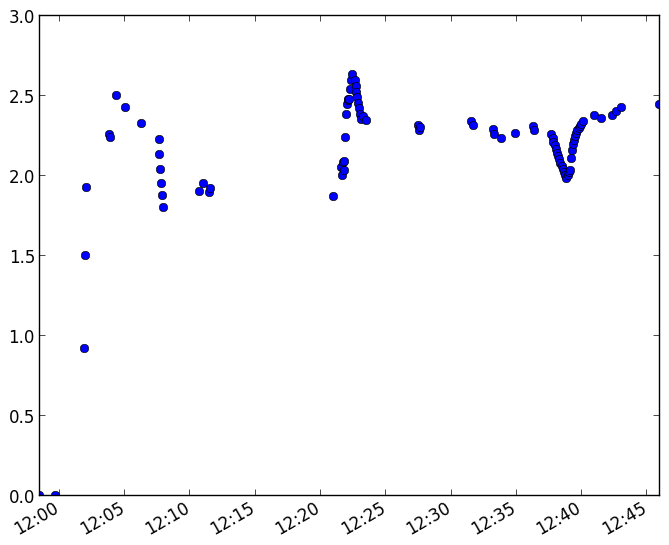
\includegraphics[scale=0.66]{../experimentacion-barbeiton/entropy_src.png}
  \caption{Entropía en función del tiempo tomando como fuente las IP source.}
\end{figure}

\begin{figure}[H]
  \centering
	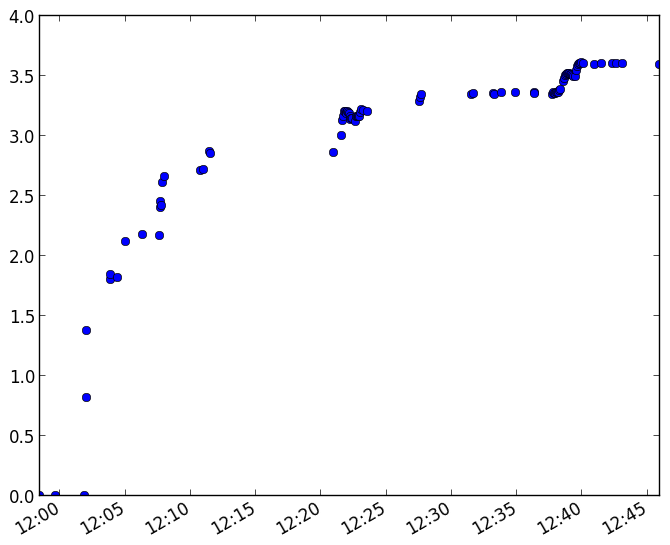
\includegraphics[scale=0.66]{../experimentacion-barbeiton/entropy_dst.png}
  \caption{Entropia de la fuente de IP destino.}
\end{figure}

\subsubsection{Conclusiones del experimento}
En la Figura $15$ podemos ver el grafo de la red según el intercambio de paquetes ARP. Se puede notar que el nodo que intercambia la mayor cantidad de paquetes ARP es el de IP número 192.168.1.1. El dispositivo con dicha IP parece estar al centro del intercambio de los paquetes ARP en la red, con lo que podemos concluir que se trata de un access point. El hecho de que este dispositivo tenga ese número de IP es una evidencia en favor de esa suposición, ya que es una dirección usual para access points.
\par Durante la hora en la cual se realizó el experimento, podemos ver que la entropía de la fuente $S_{src}$ fue variando considerablemente, aunque siempre tiende al aumento, como puede verse en la figura $16$. La entropía de la fuente de información modelada como $S_{dst}$ también tiende a aumentar, aunque de forma mucho menos errática que la anterior. 
\par En la figura $14$ podemos ver que nuevamente, el nodo con IP 192.168.1.1 se destaca con respecto a los demás. En este gráfico se muestra que la cantidad de paquetes que ARP que envía este nodo es más de $4$ veces superior a los demás nodos. 
\par Un dato interesante que surge de la figura $14$ es la aparición de la IP 0.0.0.0. Esta IP es una dirección que podría aparecer en un host cuando éste no tiene aignada una dirección de IP válida.


%\section{Conclusiones}

\end{document}
